\documentclass{article}\usepackage[]{graphicx}\usepackage[]{color}
%% maxwidth is the original width if it is less than linewidth
%% otherwise use linewidth (to make sure the graphics do not exceed the margin)
\makeatletter
\def\maxwidth{ %
  \ifdim\Gin@nat@width>\linewidth
    \linewidth
  \else
    \Gin@nat@width
  \fi
}
\makeatother

\definecolor{fgcolor}{rgb}{0.345, 0.345, 0.345}
\newcommand{\hlnum}[1]{\textcolor[rgb]{0.686,0.059,0.569}{#1}}%
\newcommand{\hlstr}[1]{\textcolor[rgb]{0.192,0.494,0.8}{#1}}%
\newcommand{\hlcom}[1]{\textcolor[rgb]{0.678,0.584,0.686}{\textit{#1}}}%
\newcommand{\hlopt}[1]{\textcolor[rgb]{0,0,0}{#1}}%
\newcommand{\hlstd}[1]{\textcolor[rgb]{0.345,0.345,0.345}{#1}}%
\newcommand{\hlkwa}[1]{\textcolor[rgb]{0.161,0.373,0.58}{\textbf{#1}}}%
\newcommand{\hlkwb}[1]{\textcolor[rgb]{0.69,0.353,0.396}{#1}}%
\newcommand{\hlkwc}[1]{\textcolor[rgb]{0.333,0.667,0.333}{#1}}%
\newcommand{\hlkwd}[1]{\textcolor[rgb]{0.737,0.353,0.396}{\textbf{#1}}}%

\usepackage{framed}
\makeatletter
\newenvironment{kframe}{%
 \def\at@end@of@kframe{}%
 \ifinner\ifhmode%
  \def\at@end@of@kframe{\end{minipage}}%
  \begin{minipage}{\columnwidth}%
 \fi\fi%
 \def\FrameCommand##1{\hskip\@totalleftmargin \hskip-\fboxsep
 \colorbox{shadecolor}{##1}\hskip-\fboxsep
     % There is no \\@totalrightmargin, so:
     \hskip-\linewidth \hskip-\@totalleftmargin \hskip\columnwidth}%
 \MakeFramed {\advance\hsize-\width
   \@totalleftmargin\z@ \linewidth\hsize
   \@setminipage}}%
 {\par\unskip\endMakeFramed%
 \at@end@of@kframe}
\makeatother

\definecolor{shadecolor}{rgb}{.97, .97, .97}
\definecolor{messagecolor}{rgb}{0, 0, 0}
\definecolor{warningcolor}{rgb}{1, 0, 1}
\definecolor{errorcolor}{rgb}{1, 0, 0}
\newenvironment{knitrout}{}{} % an empty environment to be redefined in TeX

\usepackage{alltt}
% Uncomment the following line to allow the usage of graphics (.png, .jpg)
%\usepackage[pdftex]{graphicx}
% Comment the following line to NOT allow the usage of umlauts
\usepackage[utf8]{inputenc}
\usepackage{setspace}
\usepackage{amsmath}
\usepackage{graphicx}
\title{Eviews: OLS and residual tests}
\author{Rob Hayward}
\date{}

% Start the document
\IfFileExists{upquote.sty}{\usepackage{upquote}}{}
\begin{document}
\doublespace
\maketitle
% Create a new 1st level heading
\section*{Introduction}
This paper provides a step-by-step guide to using Eviews to estimte Ordinary Least Squares and test the assumptions behind the estimation system.  The estimtion of the reltionship between the return on Bank of America and the return on the S\&P 500 is used as an example. The raw dat for the Bank of America share price and the price of the Exchange Traded Fund (ETF) that tracks the S\&P 500 are in the file BAC.csv on Student Central. 

\section*{Import data into Eviews}
Assuming that you have data in a excel file, you copy the data that you want to use and paste this into the Eviews workspace. To do this you will have to right-click the mouse and you will see the the \emph{Import data wizard} like that in Figure \ref{import}. 

\begin{figure}[h!]
\graphicspath{{"../Eviews/Figures/"}}
\centering
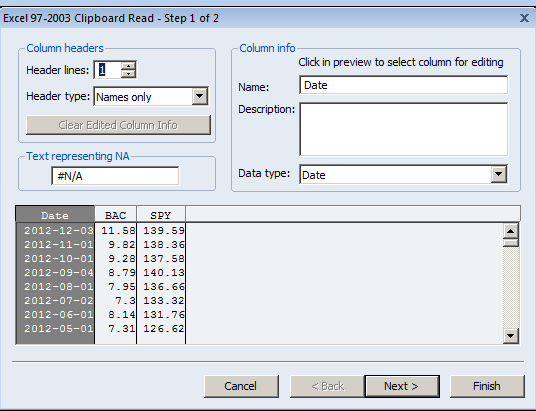
\includegraphics[height = 6cm]{Import}
\caption{Import data wizard}
\label{import}
\end{figure}

Most of the options should be cler. The main thing that you have to note is that the series that contains the information about the date should be specified.  One you have imported the data, you should have the following series: BAC, SPY and Date.  You can delete the data so long as the date has been spefified correctly and the share price numbers line up alongside the correct month.

The Eviews workspace should look like Figure \ref{WP}

\begin{figure}[h!]
\graphicspath{{"../Eviews/Figures/"}}
\centering
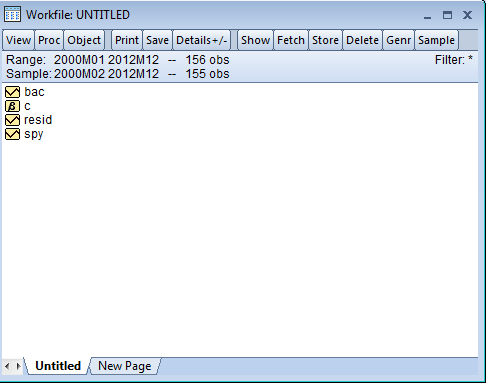
\includegraphics[height = 6cm]{Workspace}
\caption{Workspace with series added}
\label{WP}
\end{figure}

\section{Mnipulating Series}
Once you have imported the raw data series into Eviews, it is possible to create new series by manipulating the existing numbers.  This can be done in one of three ways:  Using the command line, using "Quick" and then 'Series" from the menue or Creating a new "series" "Object".  

To turn the raw share price data into returns it is necessry to calculate the percentage change in the share price each month. The special command \verb + @pch + Eviews command.  Figure \ref{RC} shows how this can be written in the command area.  The commnd 'series' will create a new series, the next element is the name and third term will specify the values 

\begin{figure}[h!]
\graphicspath{{"../Eviews/Figures/"}}
\centering
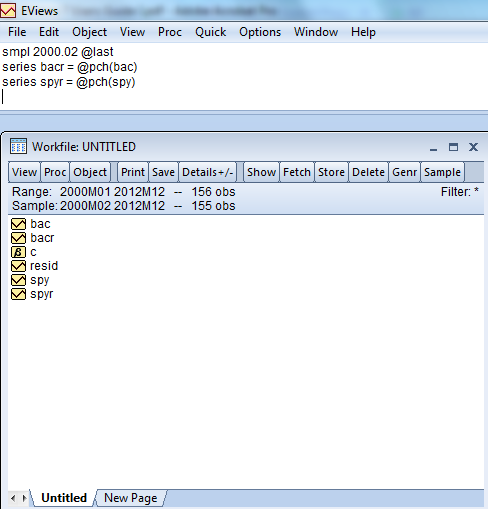
\includegraphics[height = 6cm]{Returncodefull}
\caption{Command line creation of return series}
\label{RC}
\end{figure}

\section{Estimating an equation}
Once the data have been imported and manipulated as needed the next step is to estimate the relationships between the variables.  Eviews will allow a number of different estimation techniques. However, we will use OLS.  This can be done by using the command 'equation' in the command line or 'quick-estimation' from the menu.  

Figure \ref{eq} shows the commnds for OLS with the 'eq1' the name of the equation and then the specification of the equation with the dependent variable followed by 'c' for the constant and then the explanatory variables. 

\begin{figure}[h!]
\graphicspath{{"../Eviews/Figures/"}}
\centering
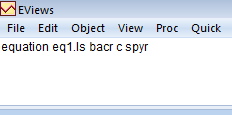
\includegraphics[height = 6cm]{equation}
\caption{Specifying the OLS equation}
\label{eq}
\end{figure}

The result of the estimation of Equation \ref{eq} is shown in Figure \ref{OLS}. The $R^2$ indicates the proportion of the change in the dependent variable that is explined by the model. In this case it is about 30\%.   

%\begin{figure}[h!]
%\graphicspath{{"../Eviews/Figures/"}}
%\centering
%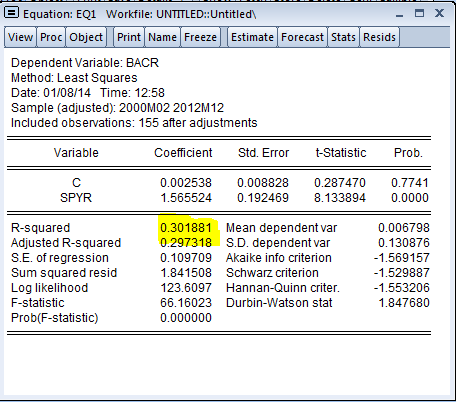
\includegraphics[height = 6cm]{eq1.r2}
%\caption{Estimted equation ouput: R squred}
%\label{OLS}
%\end{figure}



\section{Testing coefficients}
The reltionship between the dependent and explanatory varibles is estimated with some imprecison.  With different sample a different estimate would be made.  It would be useful to have some idea of the range of potentil estimates to assess whether the estimte is reliable. 
\end{document}
